\documentclass[11pt,a4paper]{article}
\usepackage{bbm,amsthm,amsfonts,amssymb,amsmath,latexsym,epic,eepic}
\usepackage{marvosym,graphicx,fancyhdr,bbm}
\usepackage[dvips]{color}
\usepackage[rflt]{floatflt}
\usepackage{colortbl}
\definecolor{Grey}{rgb}{0.5,0.5,0.5}
\definecolor{Red}{rgb}{1.0,0.0,0.0}

\usepackage{typearea}
\areaset{156mm}{235mm}
%\setlength{\parskip}{5pt plus 2pt minus 1pt}
\setlength{\parindent}{0pt}

% use \M for matrices and \V for vectors in math mode
\newcommand{\M}[1]{\mathbf{#1}}
\newcommand{\V}[1]{\mathbf{#1}}
\newcommand{\norm}[1]{\left | \left | #1 \right | \right |}
\newcommand{\RR}{\mathbbm{R}}        % set of real numbers


\renewcommand\floatpagefraction{0.8}
\renewcommand\topfraction{1}
\renewcommand\bottomfraction{0.9}
\renewcommand\textfraction{0.0}
%\def\dbltopfraction{1.0}
%\def\bottomfraction{1.0}
%\def\dblfloatpagefraction{0.8}


\makeatletter
\renewenvironment{thebibliography}[1]
     {\section*{\refname}%
      \@mkboth{\MakeUppercase\refname}{\MakeUppercase\refname}%
	 \parsep0mm
	 \itemsep0mm
	 %\labelsep0mm
	 %\itemindent0mm
      \list{\@biblabel{\@arabic\c@enumiv}}%
           {\settowidth\labelwidth{\@biblabel{#1}}%
            \leftmargin\labelwidth
            \advance\leftmargin\labelsep
            \@openbib@code
            \usecounter{enumiv}%
            \let\p@enumiv\@empty
            \renewcommand\theenumiv{\@arabic\c@enumiv}}%
      \sloppy
      \clubpenalty4000
      \@clubpenalty \clubpenalty
      \widowpenalty4000%
      \sfcode`\.\@m}
     {\def\@noitemerr
       {\@latex@warning{Empty `thebibliography' environment}}%
      \endlist}
\renewcommand\newblock{\hskip .11em\@plus.33em\@minus.07em}
\let\@openbib@code\@empty
\makeatother



\begin{document}

\title{\Large\bf Abgabe zum Praktikum Mess- und Regelungstechnik \\ \textbf{Revision 1}}

\author{Simon Klüpfel, Lukas Zeller\\
  Robotik und Telematik \\
  Universität Würzburg\\
  Am Hubland, D-97074 Würzburg\\
{\small \texttt{simon.kluepfel@stud-mail.uni-wuerzburg.de, lukas.zeller@stud-mail.uni-wuerzburg.de}}
}
\date{17. November 2022}

\maketitle

\textbf{TODO:}
\begin{verbatim}
Abstract: Zusammenfassung
Einleitung: Rando BS das zum Thema hinführt
Problembeschreibung: Warum ist lokalisierung nötig, wie das lösen (Odom+AMCL)
General Shit: Was ist unser Roboter, was ist ROS
Wie funktioiert Odom, mit Mathe und so
Gmapping kurz vorstellen, wie wir es verwenden
AMCL vorstellen, wie funktioniert es grob
Wir haben einen Pfadverfolgungs algo bekommen, wie er GROB funktioniert (Steuergesetzt sagen, macht Linie zw gegebenen Punkten)
Experimente zur bestimmung der Güte der Pfadverfolgung mit AMCL/Odom -> MESSUNGEN UNABHÄNGIG VONEINANDER!!
Zusammenfassung der Ergebnisse
Messdaten aus Exp im anhang als Tabelle
\end{verbatim}
\section{Einleitung}
Die Lokalisierung eines Roboters ist eine Problemstellung die uns im modernen, digitalen Alltag ständig begegnet. Ob es der Rasenmähroboter, die Spielzeugdrohne oder gar der mit zig Sensoren
gespickte Tesla ist, sie alle finden sich in ihrer Umgebung zurecht, oder müssen Hindernissen ausweichen, und das auch noch mit möglichst großer Präzision. Denn wer möchte schon einen 
unsauber gemähten Rasen, ein Auto was beim automatischen Einparken den Nachbarn touchiert, oder einen Multicopter der im Baum hängen bleibt? 
Durch eine geschickte Kombination aus Soft- und Hardware lassen sich diese Anwendungen jedoch heutzutage problemlos umsetzen und sind für jedermann zugänglich. 
Tesla beispielsweise konnte alleine im Jahr 2021 963.000 Fahrzeuge an Kunden ausliefern.\footnote{https://ir.tesla.com/press-release/tesla-q4-2021-vehicle-production-deliveries} 
Die Techologie ist in unserem Alltag also bereits angekommen. 




\section{Wieso brauchen wir Lokalisierung?}

\section{Kurze Einführung in den Volksbot und ROS}

\section{Odometrie, GMapping und AMCL im Überblick}

\section{Die Funktionsweise der Pfadverfolgung und ihre Güte}

\section{Experimenteller Vergleich der Qualität der Pfadverfolgung bei Verwendung von AMCL-  bzw. Odometrie-Lokalisierung}
Nun soll betrachtet werden wie genau die Lokalisierungsmethoden einen vorgegebenen Pfad verfolgen. Desweiteren soll ein Vergleich zwischen beiden Methoden angestellt werden. 
Demnach ist die Lokalisierungsmethode besser, welche in der Verwendung eine geringere Abweichung vom vorgegebenen Pfad aufweist. 
Wir gaben dem Controller hier einen Pfad vor, welcher mit Hilfe der 3D-Design-Applikation \textit{Blender} so erstellt wurde, dass er sowohl
gerade Linien als auch weiche und harte Kurven enthält. 
\begin{figure}[h]
\caption{Der Pfad, wie er in Blender erstellt wurde. Man erkennt eine Linien-struktur bestehend aus gerade und gekurvten Teilstrecken, die wie eine Autorennstrecke einen geschlossenen Pfad bilden}
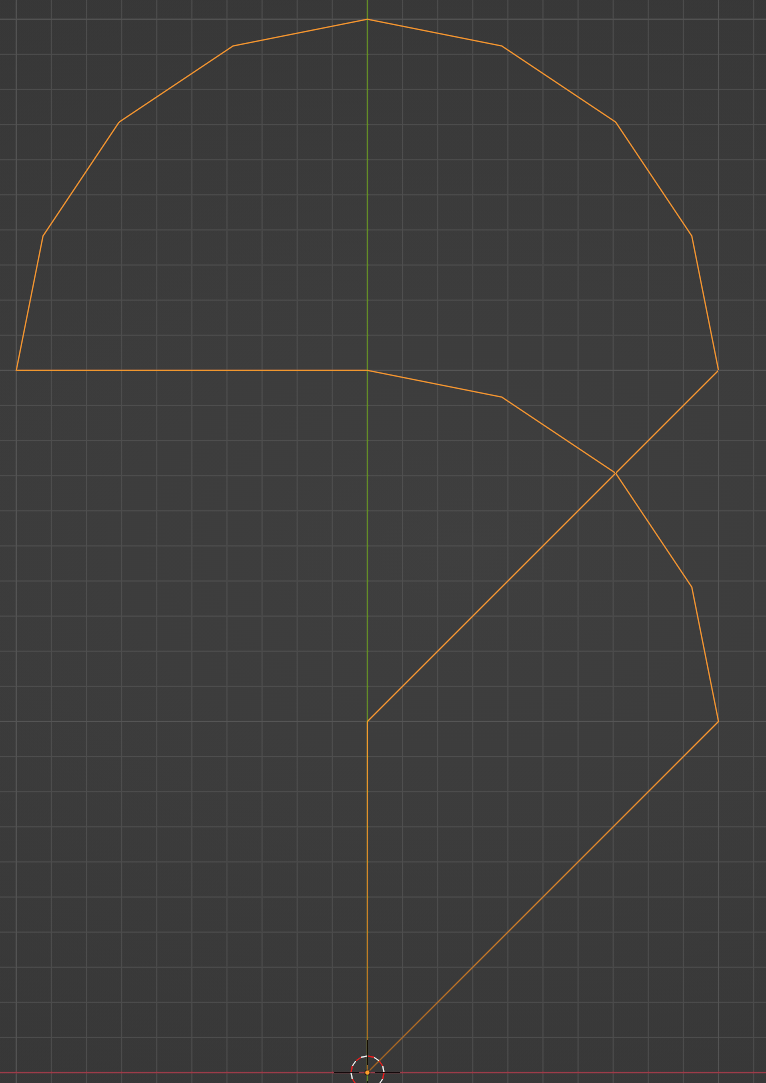
\includegraphics[height = 3cm]{pfadgrafik.png}
\end{figure}
Start und Ende sind hier der Cursor unten im Bild, Anfangsrichtung ist gerade nach oben. Die verwendete Pfaddatei ist in \verb+catkin_ws+ als 
\verb+Pfad.dat+ zu finden.
Dieser Pfad wurde auf dem Boden des Testgeländes mit Wollfäden markiert. Der Controller hat die Koordinaten des erstellten Pfades 
als relativ interpretiert. Dadurch konnten wir den Roboter am Startpunkt des Pfades platzieren, und in die Geradeaus-Richtung des Pfades orientieren. 
Dies wurde mithilfe durch ein Maßband, das durch die gerade Mittellinie des Pfades bis zum Roboter führt, und diesen dann symmetrisch teilt, möglichst exakt getan. 
Dazu wurde im Ursprung des Roboters in der Mitte der Vorderradachse ein Schraubenzieher befestigt, der gerade nach unten zeigt um die Position auf dem 
Boden leichter einsehen zu können. Es ergibt sich dennoch ein systematischer Fehler, da die Startausrichtung und -Platzierung des Roboters nicht perfekt 
mit der des Pfades am Boden übereinstimmt. Der geschätzte Maximalfehler für die Position des Roboters beträgt 2cm, der der Ausrichtung 2°. 
\\Dadurch ergibt sich im maximalen Abstand vom Startpunkt ein maximaler Fehler von: \\
$
0,02m + tan(2^\circ) * 3m = 0,12m
$                                                          \\ 
An allen anderen Orten ist der systematische Fehler durch den geringeren Abstand vom Startpunkt kleiner.
Nachdem der Roboter platziert wurde, wurde ein Node gestartet das den benannten Pfad abfährt, und dabei alle 2 Sekunden anhält, sodass seine Position 
auf dem Boden markiert werden kann. Dies wird für beide Lokalisierungsmethoden durchgeführt. Danach wird der senkrechte Abstand jedes Punktes 
zum markierten Pfad gemessen und in einer Tabelle eingetragen. Die Messergebnisse sind in Anhang\footnote{Siehe Tabelle 1} einzusehen.

\section{Beschreibung der Ergebnisse}
Der auf dem Boden markierte Pfad und die markierten Punkte, an denen der Roboter anhielt. Diese wurden jeweils auf einem Bild in Blau bei der Pfadverfolgung 
unter Verwendung von AMCL, und in Rot bei der Verwendung von Odometrie, zusätzlich zur besseren Sicht nachbearbeitet, eingekreist und mit der jeweiligen Nummer 
des Anhaltens gekennzeichnet, startend bei 0 für die Initialposition.
Man beobachtet das der Pfad anfangs, bis etwa Punkt 7, mit beiden Lokalisierungsmethoden etwa gleich gut verfolgt wird. Der Durchschnitt der Abweichungen vom Pfad 
von Haltepunkt 1 bis zu Haltepunkt 7 liegt bei Odometrie bei 8cm, bei AMCL 4,2cm. Die folgenden Punkte zeigen bei beiden Lokalisierungsmethoden eine deutlich 
größere Abweichung auf: Punkte 8-13 bei der Verwendung von Odometrie haben eine durchschnittliche Abweichung von 51,2cm, bei der Verwendung von AMCL ist bei den 
Punkten 8-14 eine durchschnittliche Abweichung von 22,9cm aufgetreten. Hierbei ist zu bemerken dass durch das beiden Ansätze in der Realität stark 
verschiedene Pfade verfolgt wurden (siehe Abbildung) und es dazu kam dass AMCL einen längeren Weg zurückgelegt hat, und somit einen Haltepunkt mehr in der Messtabelle 
aufweist als Odometrie.  Anhand der Markierungen auf dem Boden erkennt man auch dass der Odometrie-Ansatz sich nach Haltepunkt 7 durchgehend auf einer Seite des 
zu verfolgenden Pfades befindet, und immer weiter in diese Richtung von diesem abdriftet, während der AMCL Ansatz die Seite wechselt, in welche der Positionsfehler vorliegt.

\section{Diskussion und Auswertung der Fahrtwege unter AMCL und Odometrie}
Die durchschnittliche Abweichung aller Fehlerpunkte von AMCL liegt bei 12,6cm, bei der Odometrie sind es 25,9cm. Zu Beginn der Verfolgung des Pfades lagen beide Methoden 
etwa gleich nahe am Zielpfad, jedoch fing die Odometrie-Lokalisation  ab der ca. Hälfte des Pfades an eine immer größer werdende Abweichung vom Zielpfad aufzubauen bis 
zu einem maximal gemessenem Fehler von 1,13m, während bei AMCL keine größere Pfadabweichung als 36cm gemessen wurde. Das bereits beschriebene Abdriften der 
Haltepunkte des Odometrie Ansatz lässt darauf schließen das die sich akkumulierenden Fehler in den Radumdrehungen, welche das alleinige Lokalisierungsmerkmal 
der Odometrie ist, einen Drift in der Positionierung verursachen, was bewirkt das Odometrie für eine Lokalisierung auf Pfaden, die nicht kurz sind, keine der Realität 
akkuraten Ergebnisse liefern kann. Da AMCL nicht allein auf die Radumdrehungen angewiesen ist, kann es die Fehler dieser Informationsquelle ausgleichen und so auch auf 
längeren Pfaden bis zu einem gewissen Grad die Position genau bestimmen.

\section{Zusammenfassung und Ausblick}

{%\small                   % use small if you need it
\bibliographystyle{plain}
\bibliography{paper}       % use a bib-file paper.bib to collect your references
}

\end{document}

